\documentclass[text05.tex]{subfiles}
\begin{document}
\newpage
\section{アナログ入力\ruby{装置}{そう|ち}を使ってみよう}
アナログ入力\ruby{装置}{そう|ち}をHSPで使ってみましょう。A0に\ruby{感圧}{かん|あつ}センサー(\#106)をつけてください。HSPスクリプトエディタで\textasciitilde /05/anain.hspを開いて実行してみましょう。\\
\begin{figure}[H]
 \begin{minipage}[t]{0.3\columnwidth}
 \centering
 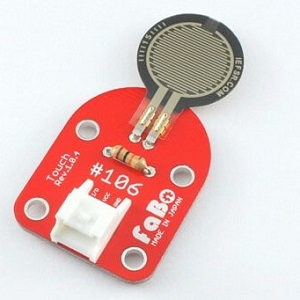
\includegraphics[width=\linewidth]{../../asset/image/text05-img021.jpg}
 \caption{\ruby{感圧}{かん|あつ}センサー}
 \end{minipage}
%\hspace{0.01\columnwidth} % ここで隙間作成
 \begin{minipage}[t]{0.5\columnwidth}
 \centering
 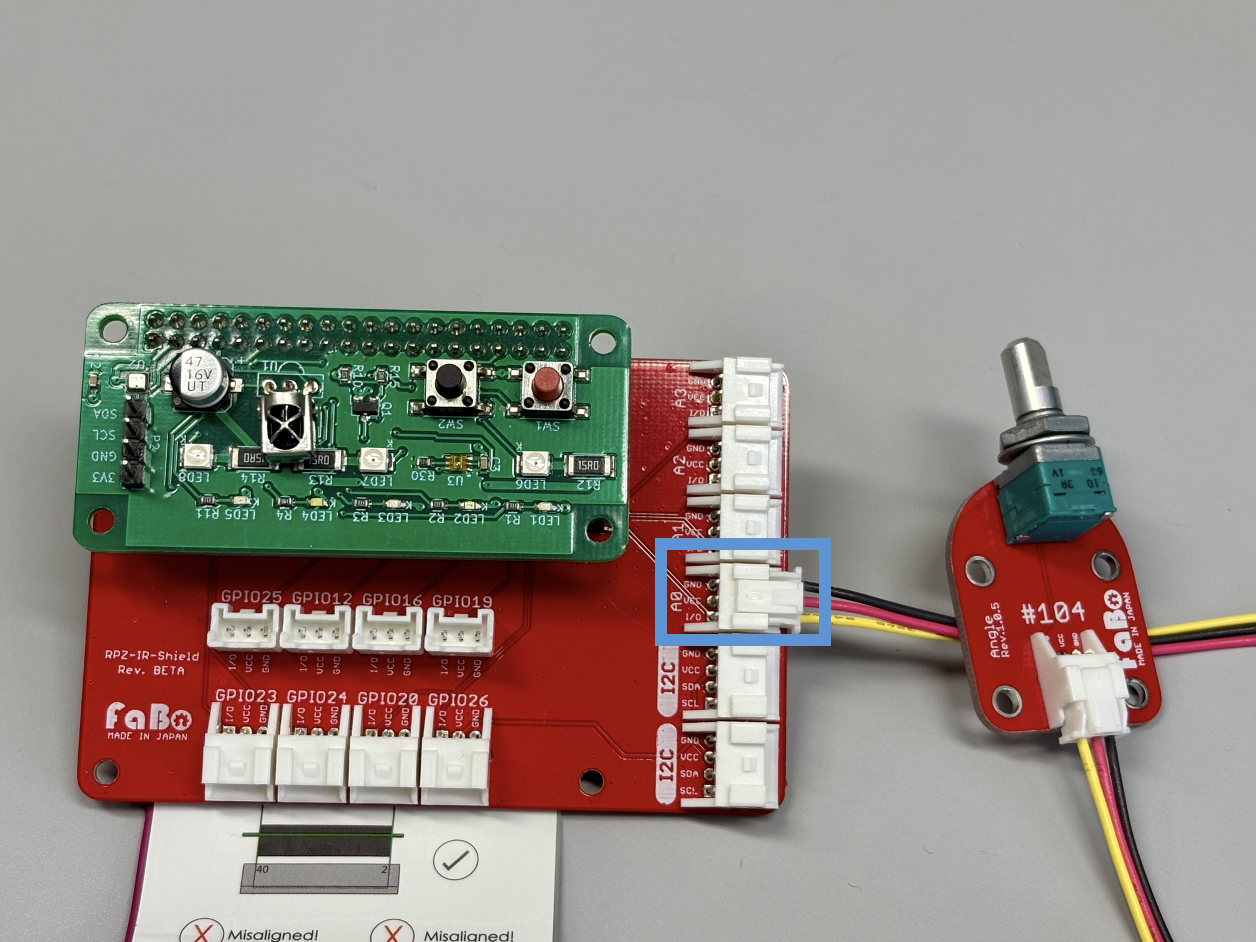
\includegraphics[width=\linewidth]{../../asset/image/text05-img030.png}
 \caption{アナログ入力A0}
 \end{minipage}
\end{figure}

\begin{lstlisting}[caption=anain.hsp,label=anain.hsp]
#include "hsp3dish.as"
#include "rpz-gpio.as"

spiopen 0	<#blue#;SPIチャンネルを開く#>

*main
	data = adcget(0,0)	<#blue#;SPIを使ってデータを受け取る#>
	res = "結果 : "+data+"\n"

	redraw 0
	pos 20,20
	font "",30
	mes res
	redraw 1

	wait 10
	goto *main

spiclose 0	<#blue#;SPIチャンネルを閉じる#>
\end{lstlisting}

anain.hspはアナログ入力\ruby{装置}{そう|ち}用のプログラムです。アナログ入力にはA0,A1,A2,A3のピンを使います。このプログラムは\ruby{感圧}{かん|あつ}センサー、ボリューム、\ruby{距離}{きょ|り}センサー、照度センサーに使うことができます。

ラズベリーパイは\ruby{一般}{いっ|ぱん}にデジタル信号しか受け付けることができません。アナログ信号をラズベリーパイが読み取れるようなデジタル信号に\ruby{変換}{へん|かん}する必要があります。その\ruby{変換}{へん|かん}のために、FaBo にはアナログ/デジタル\ruby{変換器}{へん|かん|き} (\ADC) の一種である回路が\ruby{搭載}{とう|さい}されています。\ruby{搭載}{とう|さい}されている \ADC は受け取ったアナログ信号をデジタル信号に\ruby{変換}{へん|かん}し、SPI (シリアルペリフェラルインターフェース) と\ruby{呼}{よ}ばれる\ruby{通信方式}{つう|しん|ほう|しき}を\ruby{介}{かい}して出力します。ラズベリーパイはこのデジタル信号を\ruby{解釈}{かい|しゃく}することでアナログ信号の\ruby{状態}{じょう|たい}を読み取ることができるようになります。

ラズベリーパイと HSP でアナログ信号を入力するには、まず SPI で通信するための\ruby{準備}{じゅん|び}をします。
\code{spiopen} を使います。
\code{spiopen 0} と書くと、0 番目の SPI \ruby{通信経路}{つう|しん|けい|ろ}を\ruby{準備}{じゅん|び}します。
次に、\code{\adcget} 命令で \ADC からの信号を読み取ります。 
\code{\adcget(0,0)} と書くと、A0 \ruby{端子}{たん|し}の信号を、0 番目の SPI \ruby{通信経路}{つう|しん|けい|ろ}から読みこみます。入力される\ruby{値}{あたい}は $0$ から $1023$ までの\ruby{数値}{すう|ち}になります。
\code{spiclose(0)} と書くと、0 番目の SPI \ruby{通信経路}{つう|しん|けい|ろ}を\ruby{解放}{かい|ほう}し、他の SPI 通信に\ruby{再利用}{さい|り|よう}できるようになります。
ここまでの命令をまとめます。

% TODO: 命令解説環境を作る。
\begin{itemize}
\item \code{spiopen(<通信経路番号>)}: <\ruby{通信経路}{つう|しん|けい|ろ}番号> で指定された SPI \ruby{通信経路}{つう|しん|けい|ろ}を\ruby{準備}{じゅん|び}する。\code{\adcget} 命令を使う前に\ruby{呼}{よ}び出す。
\item \code{\adcget(<ピン番号>, <通信経路番号>)}: <\ruby{通信経路}{つう|しん|けい|ろ}番号> で指定された SPI \ruby{通信経路}{つう|しん|けい|ろ}を\ruby{介}{かい}して <ピン番号> に入力するアナログ信号を読み\ruby{込}{こ}む。$0$ から $1023$ までの\ruby{数値}{すう|ち}が返る。
\item \code{spiclose(<通信経路番号>)}: <\ruby{通信経路}{つう|しん|けい|ろ}番号> で指定された SPI \ruby{通信経路}{つう|しん|けい|ろ}を\ruby{解放}{かい|ほう}する。
\end{itemize}

\ruby{授業}{じゅ|ぎょう}内の\ruby{演習}{えん|しゅう}では \ADC だけが SPI 通信を行うので、<\ruby{通信経路}{つう|しん|けい|ろ}番号> は\ruby{常}{つね}に 0 を\ruby{設定}{せっ|てい}しておいて\ruby{構}{かま}いません。
課外で他の SPI 通信をする回路を\ruby{複数}{ふく|すう}同時に使用したい場合は、<\ruby{通信経路}{つう|しん|けい|ろ}番号> が\ruby{重複}{ちょう|ふく} しないように\ruby{設定}{せっ|てい}しましょう。

アナログ入力\ruby{装置}{そう|ち}には、ボリュームや\ruby{感圧}{かん|あつ}センサなどいくつか種類があります。それぞれの具体的な使い方は\pageref{analog_in}ページを見てみましょう。\\

\begin{tcolorbox}[title=\useOmetoi]
\begin{enumerate}
\addex{\ruby{感圧}{かん|あつ}センサー(\#106)をA0につなげて上記のanain.hspを実行してみましょう。\ruby{感圧}{かん|あつ}センサーにさわる強さによって、画面の数字が変わります。}
\addex{ボリューム(\#104)をA0につなげてanain.hspを実行してみましょう。ボリュームを動かすと、画面の数字が変わります。}
\addex{照度センサー(\#109)をA0につなげてanain.hspを実行してみましょう。明るさによって、画面の数字が変わります。}
\addex{\code{\adcget(0,0)}を\code{\adcget(1,0)}に変えましょう。A1にアナログ入力そうちをつなぎましょう。anain.hspを実行してみましょう。}
\end{enumerate}
\end{tcolorbox}
\end{document}
